% Task 4: two real collisions. Which digests match is the answer, so the figure shows question marks.
\documentclass[12pt,tikz,border=6pt]{standalone}
% Shared preamble of the task figures of Lecture 7. The colours are the colour roles of the slides
% (main.tex) and of the passwords simulator:
%   Alice sIndigo, Mallory sPink, message / document / password sViolet, salt sAmber,
%   Bob / the server / the notary sTeal, digest sBrown; mechanisms dark; the unknown: orange dashed.
\usepackage{lmodern}
\usepackage[T1]{fontenc}
\renewcommand{\familydefault}{\sfdefault}
\usepackage{amsmath,amssymb}
\usepackage{xcolor}
\usepackage{fontawesome5}
\usetikzlibrary{arrows.meta, calc, positioning, fit, decorations.pathreplacing, backgrounds}

\definecolor{DeepBlue}{HTML}{283593}
\definecolor{AccentOrange}{HTML}{EB5A14}
\definecolor{nInk}{HTML}{37474F}
\definecolor{nLine}{HTML}{90A4AE}
\definecolor{nLight}{HTML}{CFD8DC}
\definecolor{nFill}{HTML}{ECEFF1}
\definecolor{aExec}{HTML}{43A047}
\definecolor{aWrite}{HTML}{E53935}
\definecolor{sIndigo}{HTML}{5C6BC0}
\definecolor{sPink}{HTML}{EC407A}
\definecolor{sViolet}{HTML}{7E57C2}
\definecolor{sAmber}{HTML}{FFB300}
\definecolor{sTeal}{HTML}{26A69A}
\definecolor{sBrown}{HTML}{8D6E63}
\definecolor{sPinkText}{HTML}{C2185B}
\definecolor{sAmberText}{HTML}{A06A00}
\definecolor{sTealText}{HTML}{00796B}

\tikzset{
  hw/.style={draw=nLine, thick, fill=nFill, text=nInk, rounded corners=3pt, align=center, inner sep=4pt},
  mech/.style={draw=nInk, thick, fill=nInk, text=white, rounded corners=3pt, align=center, inner sep=5pt, font=\small\bfseries},
  msgval/.style={draw=sViolet, thick, fill=sViolet!12, text=nInk, rounded corners=3pt, align=center, inner sep=4pt},
  saltval/.style={draw=sAmber, thick, fill=sAmber!25, text=nInk, rounded corners=3pt, align=center, inner sep=4pt},
  digval/.style={draw=sBrown, thick, fill=sBrown!15, text=nInk, rounded corners=3pt, align=center, inner sep=4pt},
  srvval/.style={draw=sTeal, thick, fill=sTeal!15, text=nInk, rounded corners=3pt, align=center, inner sep=4pt},
  unk/.style={draw=AccentOrange, thick, dashed, fill=white, text=AccentOrange, rounded corners=3pt, align=center,
    inner sep=4pt, font=\bfseries},
  data/.style={-{Stealth}, very thick, nInk},
  person/.style={circle, fill=#1, draw=#1, text=white, minimum size=1.1cm, font=\Large, inner sep=0pt},
}
\newcommand{\personnode}[4]{%
  \node[person=#3] (#1) at (#2) {\faUser};
  \node[font=\small\bfseries, text=#3, below=0.06cm of #1] (#1lbl) {#4};}
\newcommand{\mallorynode}[2]{%
  \node[person=sPink] (#1) at (#2) {\faUserSecret};
  \node[font=\small\bfseries, text=sPinkText, below=0.06cm of #1] (#1lbl) {Mallory};}
\newcommand{\hashbox}[4]{\node[mech, minimum width=#4] (#1) at (#2) {\faCogs\ #3};}

\begin{document}
\pagecolor{white}
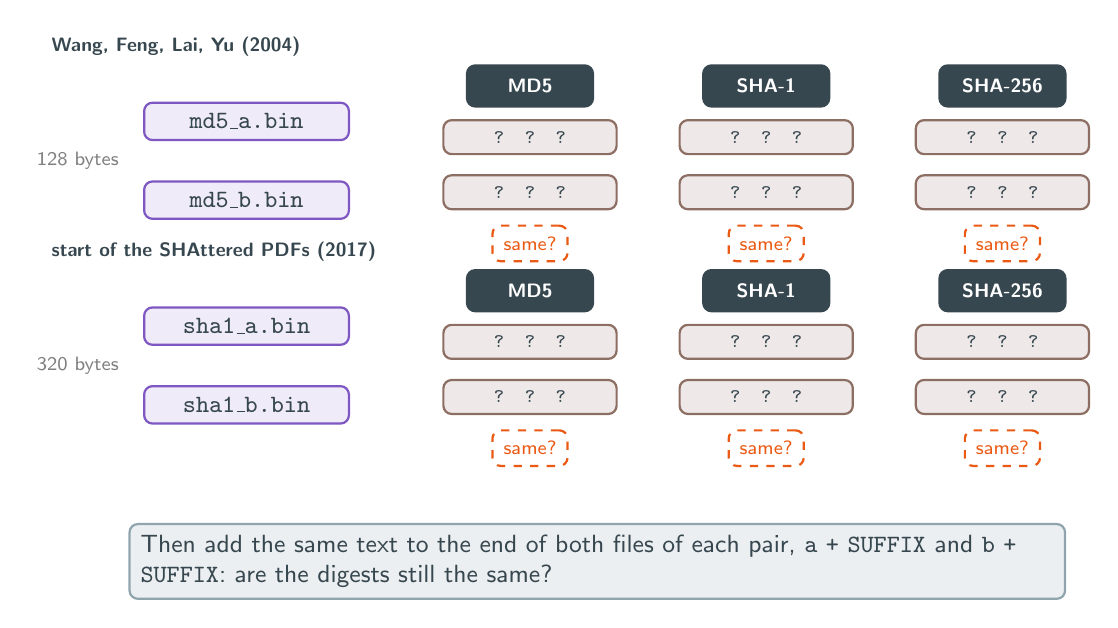
\begin{tikzpicture}[>=Stealth]
  \foreach \row/\a/\b/\n/\src in {0/md5\_a.bin/md5\_b.bin/128 bytes/{Wang, Feng, Lai, Yu (2004)}, -2.6/sha1\_a.bin/sha1\_b.bin/320 bytes/{start of the SHAttered PDFs (2017)}} {
    \node[msgval, font=\small\ttfamily, minimum width=2.6cm] (a) at (0,\row+0.5) {\a};
    \node[msgval, font=\small\ttfamily, minimum width=2.6cm] (b) at (0,\row-0.5) {\b};
    \node[font=\scriptsize, text=gray, anchor=east] at (-1.5,\row) {\n};
    \node[font=\scriptsize\bfseries, text=nInk, anchor=west] at (-2.6,\row+1.45) {\src};
    \foreach \h/\x in {MD5/3.6, SHA-1/6.6, SHA-256/9.6} {
      \node[mech, font=\scriptsize\bfseries, minimum width=1.6cm] at (\x,\row+0.95) {\h};
      \node[digval, font=\scriptsize\ttfamily, minimum width=2.2cm] at (\x,\row+0.3) {? ? ?};
      \node[digval, font=\scriptsize\ttfamily, minimum width=2.2cm] at (\x,\row-0.4) {? ? ?};
      \node[unk, font=\scriptsize] at (\x,\row-1.05) {same?};
    }
  }
  \node[hw, font=\small, text width=11.6cm, align=left, anchor=north west] at (-1.5,-4.6) {Then add the same text to the end of both files of each pair, \texttt{a + SUFFIX} and \texttt{b + SUFFIX}: are the digests still the same?};
\end{tikzpicture}
\end{document}
